
%(BEGIN_QUESTION)
% Copyright 2007, Tony R. Kuphaldt, released under the Creative Commons Attribution License (v 1.0)
% This means you may do almost anything with this work of mine, so long as you give me proper credit

A byproduct of the {\it kraft process} used in the paper industry for turning wood chips into pulp is a liquid called {\it black liquor}.  This liquid contains many volatile sulfur compounds such as hydrogen sulfide (H$_{2}$S) and mercaptans, both of which are strongly scented, and if released to the atmosphere will constitute a hazardous (or at least strongly objectionable) emission.  Loss of volatile sulfur compounds also constitutes a loss of sulfur, which is a raw material in the kraft pulping process.

These sulfur compounds may be stabilized for less volatility and easier recovery by a process of oxidation: exposing the black liquor to pure oxygen gas.  To minimize consumption of oxygen, the gas flow is metered proportionately to liquor flow:

$$\includegraphics[width=15.5cm]{i01733x01.eps}$$

Explain how this is an example of {\it ratio control}, and identify the following about the system:

\begin{itemize}
\item{} Which flow stream is the ``wild'' flow?
\item{} Which flow stream is the ``captive'' flow?
\item{} What is the purpose of the ``hand controller'' (HC)?
\item{} What factor(s) dictate the setting of the hand controller's output?
\item{} What safety hazards accompany the use of pure oxygen as a process stream?
\end{itemize}

\vskip 20pt \vbox{\hrule \hbox{\strut \vrule{} {\bf Suggestions for Socratic discussion} \vrule} \hrule}

\begin{itemize}
\item{} Identify some hazards associated with this process, given the types of substances going in and out of the reactor.
\item{} For those who have studied flow measurement, explain the siginficance of the ``square root'' symbols attached to each flow transmitter.
\item{} Explain what would happen in this process if the liquor flow transmitter failed with a low signal.
\item{} Explain what would happen in this process if the liquor flow transmitter failed with a high signal.
\item{} Explain what would happen in this process if the oxygen flow transmitter failed with a low signal.
\item{} Explain what would happen in this process if the oxygen flow transmitter failed with a high signal.
\item{} Explain what would happen in this process if the control valve failed fully shut.
\item{} Explain what would happen in this process if the control valve failed wide-open.
\end{itemize}

\underbar{file i01733}
%(END_QUESTION)





%(BEGIN_ANSWER)

\noindent
{\bf Partial answer:}

\vskip 10pt

\begin{itemize}
\item{} Which flow stream is considered the ``wild'' flow? {\it The black liquor flow.}
\item{} What safety hazards accompany the use of pure oxygen as a process stream? {\it Any and all flammable materials must be kept out of the oxygen piping and valving!}
\end{itemize}

%(END_ANSWER)





%(BEGIN_NOTES)

\begin{itemize}
\item{} Which flow stream is considered the ``wild'' flow? {\it The black liquor flow.}
\item{} Which flow stream is the ``captive'' flow? {\it The oxygen flow.}
\item{} What is the purpose of the ``hand controller'' (HC)? {\it To provide an operator-adjustable multiplier value for ratio control.}
\item{} What factor(s) dictate the setting of the hand controller's output? {\it The concentration of sulfur compounds in the black liquor.}
\item{} What safety hazards accompany the use of pure oxygen as a process stream? {\it Any and all flammable materials must be kept out of the oxygen piping and valving!}
\end{itemize}


\vskip 20pt \vbox{\hrule \hbox{\strut \vrule{} {\bf Virtual Troubleshooting} \vrule} \hrule}

This question is a good candidate for a ``Virtual Troubleshooting'' exercise.  Presenting the diagram to students, you first imagine in your own mind a particular fault in the system.  Then, you present one or more symptoms of that fault (something noticeable by an operator or other user of the system).  Students then propose various diagnostic tests to perform on this system to identify the nature and location of the fault, as though they were technicians trying to troubleshoot the problem.  Your job is to tell them what the result(s) would be for each of the proposed diagnostic tests, documenting those results where all the students can see.

During and after the exercise, it is good to ask students follow-up questions such as:

\begin{itemize}
\item{} What does the result of the last diagnostic test tell you about the fault?
\item{} Suppose the results of the last diagnostic test were different.  What then would that result tell you about the fault?
\item{} Is the last diagnostic test the best one we could do?
\item{} What would be the ideal order of tests, to diagnose the problem in as few steps as possible?
\end{itemize}


\vfil \eject

\noindent
{\bf Summary Quiz:}

Identify the consequence of the liquor flow transmitter failing with a low signal, so that it outputs nearly 4 mA of loop current even with a normal flow rate of black liquor into the reactor vessel:

$$\includegraphics[width=15.5cm]{i01733x01.eps}$$

\begin{itemize}
\item{} The black liquor flow will dramatically increase
\vskip 5pt 
\item{} The output liquor will be excessively oxidized
\vskip 5pt 
\item{} The oxygen will cavitate as it passes through the valve
\vskip 5pt 
\item{} The oxygen flow transmitter will also fail low
\vskip 5pt 
\item{} The output liquor will be insufficiently oxidized
\vskip 5pt 
\item{} The black liquor flow will dramatically decrease
\end{itemize}

%INDEX% Control, strategies: ratio
%INDEX% Process: black liquor oxidation (Kraft pulping)

%(END_NOTES)


